%---------------------------------------------------------------------------------
\chapter{Numerical methods}
\label{chap:numerical-methods}
%---------------------------------------------------------------------------------
\section{Ordinary differential equation}
An Ordinary Differential Equation(ODE) is an equation that contains derivatives of single independent variable functions. For example, $\frac{df}{dt}=-t$ and $\frac{df}{dt} + \frac{dg}{dt} = 4t$. 

In general, ODEs are used to describe changes, the simplest example is speed where it is the change in distance travelled. ODEs are also widely used in biological problem. For example, the SEIR model that describes the spread of a disease in a population. It compartmentalise the population into groups of Susceptibles, Exposed, Infectious and Recovered. Transition of individuals from groups is described by a system of ODEs. It is defined as 
\begin{align}
\label{model:SEIR}
    \frac{dS(t)}{dt} &= -\beta S(t)I(t), \\
    \frac{dE(t)}{dt} &= \beta S(t)I(t) - \kappa E(t), \\
    \frac{dI(t)}{dt} &= \kappa E(t) - \gamma I(t), \\
    \frac{dR(t)}{dt} &= \gamma I(t)
\end{align}
where $S$, $E$, $I$ and $R$ are susceptible, exposed, infectious and recovered individuals, while parameters $\beta$, $\kappa$ and $\gamma$ are infection rate, incubation rate and recovery rate respectively. Figure \ref{fig:SEIR_simulation} shows the incidence cases simulated by the ODE system. 

\begin{figure}
    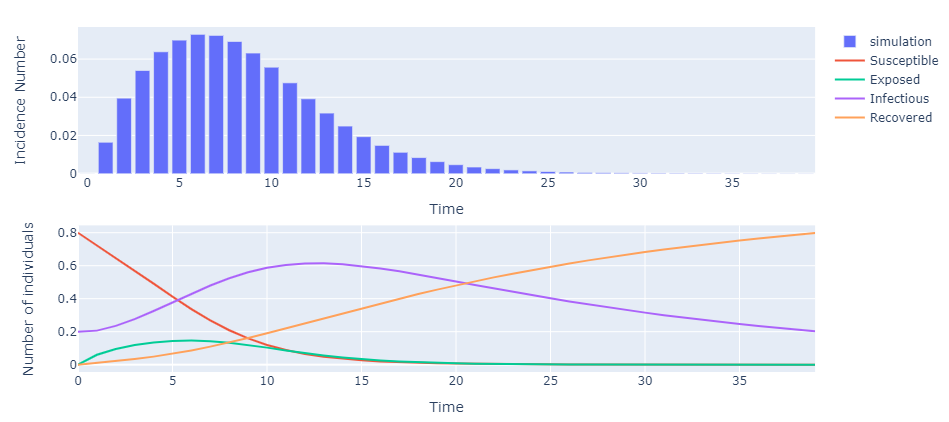
\includegraphics[width=0.95\columnwidth]{SEIR_simulation.png}
    \caption{Simulation of the SEIR model. The bar graph shows the incidence number, while the line graph shows the number of individuals in each group.}
    \label{fig:SEIR_simulation}
\end{figure}

Another example is the modelling of excitable systems, such as the heart muscle cells and nerve cells. The Hodgkin \& Huxley model models the ionic currents across the cell membrane, to explain the action potential of nerve cells.%\cite{math_physio}
Their model is defined as
\begin{equation}
\label{model:HH}
    C_m \frac{dV}{dt} = -g_{\text{eff}}(V - V_{\text{eq}}) + I_{\text{app}} \\
\end{equation}
where $C_m$ is membrane capacitance, $V$ is membrane potential, $g_{\text{eff}}$ is sum of conductance for all ion channels, $V_{\text{eq}}$ is membrane resting potential and $I_{\text{app}}$ is applied current. Figure \ref{fig:AP_simulation} shows the simulated action potential of Hodgkin and Huxley model.

\begin{figure}
\centering
    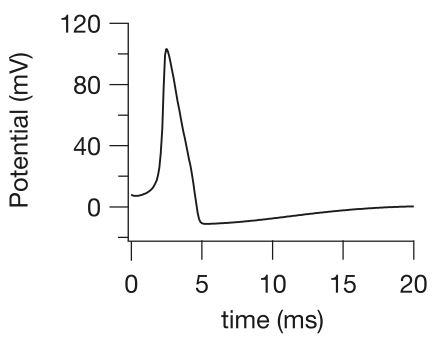
\includegraphics[width=0.4\columnwidth]{AP_simulation}
    \caption{Action potential in Hodgkin and Huxley model, adapted from \hl{to cite math physio}.}
    \label{fig:AP_simulation}
\end{figure}

\section{Initial value problem}
To solve these ODEs, initial conditions are required to \hl{specify a value of the functions at a certain point in the domain}, as there are infinitely possible solutions to ODE. The initial condition could then \hl{restrict the solutions to a single one that we are interested in}. The ODEs, together with its initial conditions, \hl{construct the initial value problem}.

A general form of an initial value problem is as follows: 
\begin{align}
    y'&=f(x,y)\\
    y(x_0) &= y_0 \label{eqn:initial_value}
\end{align}
for $x \in [x_0, X_M]$, where (\ref{eqn:initial_value}) is the initial condition that restricts the solution. The definition provided in SEIR Model \ref{model:SEIR}, with given parameter values, is not sufficient to solve the model. The initial values chosen to plot Figure \ref{fig:SEIR_simulation} are $S(0)=0.8, E(0)=0, I(0)=0.1$ and $R(0)=0$.

\section{Numerical method}
In general, ODE system cannot be solved analytically, for example the given models SEIR Model \ref{model:SEIR} and Hodgkin \& Huxley Model \ref{model:HH}. Therefore, the solution has to be estimated by numerical methods. The most popular and simple method is the Euler's method.

Intuitively, Euler's explicit method assumes for a small step size, the solution of the function can be estimated by its tangent line. As seen in Figure \ref{fig:Euler_method}, at point $x_1$, the change in height from $x_0$ to $x_1$ is $hF(x_0,y_0)$. So, we have the estimated value of $y_1$ to be $y_0 + hF(x_0,y_0)$, where $y_0$ is the value of solution curve at $x_0$.

\begin{figure}
\centering
    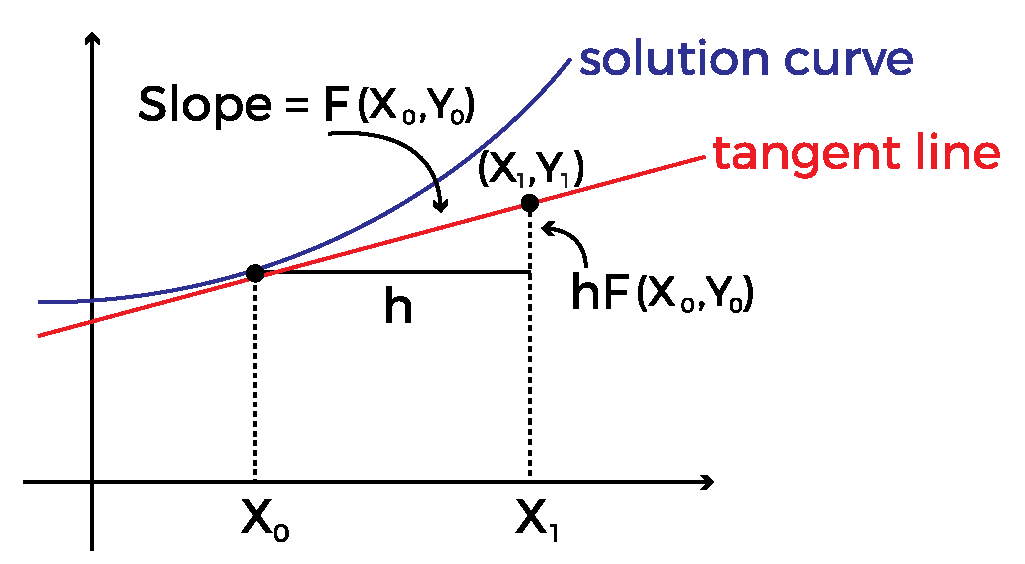
\includegraphics[width=0.5\columnwidth]{Euler_method_img}
    \caption{Intuition of Euler's method, adapted from \hl{https://calcworkshop.com/first-order-differential-equations/eulers-method-table/}}
    \label{fig:Euler_method}
\end{figure}

\section{One-step methods}
\label{sec:one-step-method}
Throughout the report, the following notation will be used:
\begin{itemize}
    \item $y_n$ - numerical approximation of $y(x_n)$
    \item $y(x_n)$ - analytical solution at mesh point $x_n$
    \item $x_n$ - mesh points of defined range, where
\end{itemize}

\begin{align}
    x_n &= x_0 + nh\\
    h &= \frac{(X_M - x_0)}{N}
\end{align}
for $n = 0,\dots, N$.

Euler's explicit method has the following definition,  
\begin{equation}
    y_{n+1} = y_n + hf(x_n,y_n)\\
\end{equation}
Starting from the initial value, the solution at the subsequent mesh point is estimated to follow a straight line with gradient as given.

The implementation is as follows:

\begin{algorithm}[H]
    \SetAlgoLined
    \SetKwInOut{Output}{Output}
    \Output{mesh points and its numerical solution}
    solution = [initial value]\;
    meshpoints = [starting point]\;
    \For{$n$ \text{from} 1 \text{to total number of mesh points}}{
    solution.append(solution[$n-1$] + step size * $f$(meshpoints[$n-1$], solution[$n-1$])\;
    meshpoints.append(meshpoints[$n-1$] + $n$ * step size)\;
    }
    \Return{meshpoints and solution}\;
\caption{Euler's explicit method}
\end{algorithm}

A vector of numerical solution and a vector of mesh points are initialised with their respective initial values. At each iteration, the mesh point and the numerical solution at the mesh point are calculated. The series of mesh points and its solution are returned. \hl{The mesh points are returned so that the users does not have to keep track of the specifications they used. Moreover, for consistency of the solver, all implemented methods will return the mesh points used and its solution. In adaptive methods, the output of mesh points would be important to know the position of the solution.}

The truncation error of Euler's explicit method is defined to be the difference between the exact solution and the numerical solution given the exact solution of previous mesh point is known. We have that the truncation error for Euler's explicit method is

\begin{equation}
\label{eqn:trun_err_def}
    T_n \defeq \frac{y(x_{n+1}) - y(x_{n})}{h} - f(x_n, y(x_n))
\end{equation}
According to Taylor's series expansion, we have 
\begin{equation}
\label{eqn:Taylor_expansion}
    y(x_n + h) = y(x_n) + hy'(x_n) + \frac{1}{2}hy''(\xi_n)
\end{equation}
for some $\xi_n \in (x_n, x_{n+1})$. Substitute (\ref{eqn:Taylor_expansion}) to (\ref{eqn:trun_err_def}), noting that $f(x_n, y(x_n)) = y'(x_n)$, we get
\begin{equation}
    T_n = \frac{1}{2}hy''(\xi_n)
\end{equation}
Therefore, the truncation error for Euler's explicit method varies linearly with the step size.

An example model 
\begin{align}
\label{eqn:example_model}
    f(x,y) &= -y \\
    y(0) &= 1
\end{align}
for $x \in [0, 5]$ is used throughout this report to check that the implementation follows the theory. The analytical solution to this problem is $y = e^{-x}$. Some examples of the solution to the given example model (\ref{eqn:example_model}) can be found via this link: \href{https://nbviewer.jupyter.org/github/FarmHJ/numerical-solver/blob/main/examples/solver_convergence.ipynb}{\underline{\emph{example model notebook}}}.

\hl{Taking the example model} \ref{eqn:example_model} \hl{as a reference}, the truncation error vs step size graph is shown in Figure \ref{fig:Euler_explicit_error_behaviour}. The truncation error is computed by taking the difference between the exact solution and the numerical solution at a randomly chosen $x$ value of 3 for the example model \ref{eqn:example_model}. The truncation error is computed for different step sizes, where the computation of numerical solution is repeated. Figure \ref{fig:Euler_explicit_error_behaviour} is plotted in logarithmic scale for both variables. It can be observed that $\log |T_n|$ increases linearly with $\log h$, same as the theoretical prediction. 

\begin{figure}
    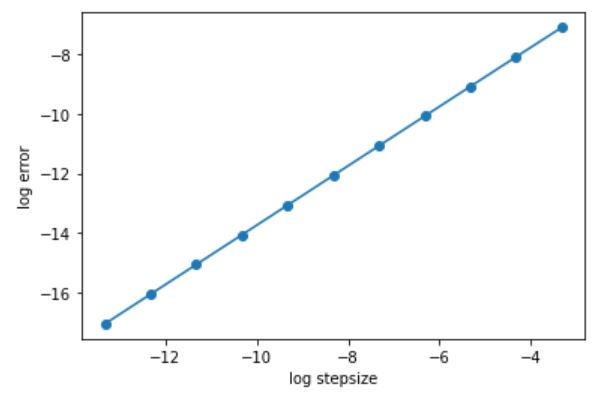
\includegraphics[width=0.95\columnwidth]{Euler_explicit_error_behaviour}
    \caption{Truncation error of Euler's explicit method for various step sizes.}
    \label{fig:Euler_explicit_error_behaviour}
\end{figure}

Other than Euler's explicit method, the other one-step methods implemented are Euler's implicit method, the trapezium rule method and the four-stage explicit Runge-Kutta method. Euler's implicit method is defined to be
\begin{equation}
    y_{n+1} = y_n + hf(x_{n+1},y_{n+1}),\\
\end{equation}
while the trapezium rule method is
\begin{equation}
    y_{n+1} = y_n + \frac{1}{2}h[f(x_n,y_n) + f(x_{n+1},y_{n+1})].\\
\end{equation}
The definition of the four-stage Runge-Kutta method is
\begin{equation}
    y_{n+1} = y_n + \frac{1}{6}h(k_1 + 2k_2 + 2k_3 + k4)
\end{equation}
where
\begin{align}
    k_1 &= f(x_n, y_n) \\
    k_2 &= f(x_n + \frac{1}{2}h, y_n + \frac{1}{2}hk_1) \\
    k_3 &= f(x_n + \frac{1}{2}h, y_n + \frac{1}{2}hk_2) \\
    k_4 &= f(x_n + h, y_n + hk_3).
\end{align}

Using the same definition for truncation error in \ref{eqn:trun_err_def}, we have that the truncation error of Euler's implicit method, trapezium rule method and four-stage Runge-Kutta method are $T_n = -\frac{1}{2}hy''(\xi_n)$ for $\xi_n \in (x_n, x_{n+1})$, $T_n = -\frac{1}{12}h^2y^{(3)}(\xi_n)$ for $\xi_n \in (x_n, x_{n+1})$ and $T_n = \mathcal{O}(h^4)$ respectively.

When these methods are tested on the example model \ref{eqn:example_model}, the truncation error does not behave as expected, as shown in the graph below. This is probably due to the use of fixed point iteration algorithm to estimate the solution of implicit functions. The error of the fixed point iteration algorithm might be added to the error of the numerical method. Therefore, the difference of the numerical solution with the exact solution is larger for implicit methods as compared to Euler's explicit methods.

These methods are tested on the example model \ref{eqn:example_model}, the truncation error behaviour graph is shown in Figure \ref{fig:onestep_error_behaviour}. Since the graph is plotted in logarithmic scale, the gradient of the lines shows the order of accuracy of the methods. The truncation error behaviour of Euler's implicit method overlaps \hl{that of} Euler's explicit method. The gradient for Euler's explicit, Euler's implicit and the trapezium rule method are 1, 1 and 2 respectively. \hl{RK4}

\begin{figure}
    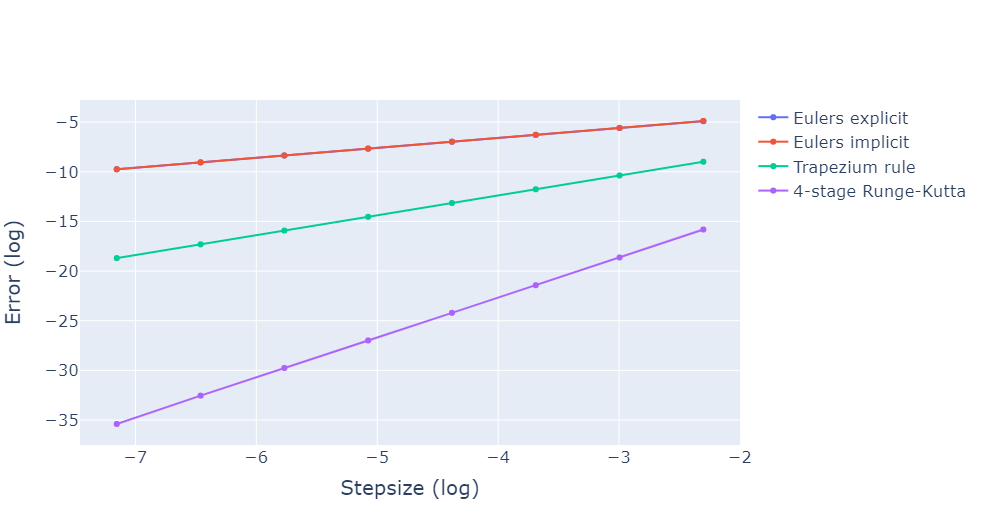
\includegraphics[width=0.95\columnwidth]{onestep_error_behaviour}
    \caption{Truncation error of Euler's implicit method and trapezium rule method for various step sizes.}
    \label{fig:onestep_error_behaviour}
\end{figure}

\section{Predictor-corrector methods}
\label{sec:predictor-corrector}
For the implicit one-step methods, numerical value at previous mesh point is chosen as the initial guess for the fixed point iteration algorithm. The predictor-corrector method suggests a more carefully chosen initial guess for the implicit methods. An explicit numerical method is used as a predictor for the initial guess of an implicit method. The initial value is then used for the iterations in the algorithm to solve an implicit function. The implicit method that refines the solution is known as the corrector method. 

The Euler-Trapezoidal method is a predictor-corrector that uses an Euler's explicit method as the predictor and trapezium rule method as the corrector. In this implementation, the trapezium rule method corrector is iterated until a set of conditions are satisfied. The conditions are set to be the difference between current iteration and previous iteration is lesser than a given threshold value or the number of iterations exceeds a certain amount. The figure below shows the graph of $\log |T_n|$ against $\log h$.

\begin{figure}
    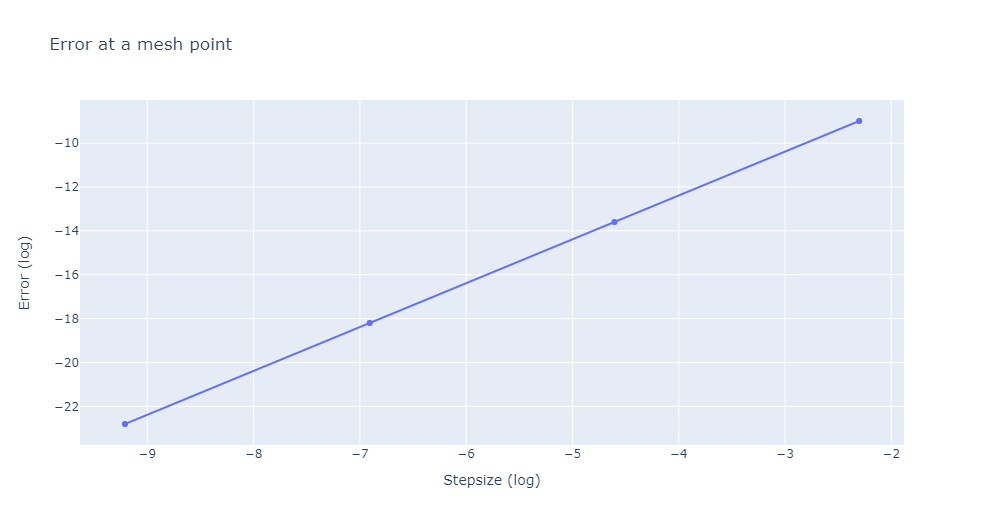
\includegraphics[width=0.95\columnwidth]{predictor_corrector_error_behaviour}
    \caption{Error of Euler-Trapezoidal method for various step sizes.}
    \label{fig:predictor_corrector_error_behaviour}
\end{figure}

\section{Adaptive method}
\label{sec:adaptive-method}
In some types of problem, the solution to the problem exhibits a behaviour where step sizes have to be sufficiently small for a stable solution. In other words, the solution have small changes with mesh points. Such problems are called stiff problems. In order to obtain a stable solution, the computational cost is high. Moreover, such a stable solution would have resolution higher than that required for practical purposes.

Adaptive methods focus on achieving the desired accuracy with low computational cost. The main idea of an adaptive method is to control the precision at each mesh point. The error at each mesh point is estimated. If the error is larger than a threshold value, a smaller step size is chosen. These steps are repeated until the error is smaller than the given threshold value.

The adaptive method implemented in this software is based on the BS23 (Bogacki and Shampine) and RKF45 (Runge-Kutta-Fehlberg) method. A lower order method is used to estimate the solution, while a higher order method is used to estimate the error. 

Absolute tolerance and relative tolerance were used in the implementation of the adaptive methods. Similarly, the implemented adaptive method is used to solve the example model \ref{eqn:example_model}. The adaptive methods were tested for convergence. Two comparisons were made, one based on absolute tolerance and the other on relative tolerance. As shown in Figures \ref{fig:ode45_absolute_sum_error_behaviour} and \ref{fig:ode45_relative_sum_error_behaviour}, the error of the method is smaller for smaller tolerance, regardless of absolute tolerance or relative tolerance.

\begin{figure}
    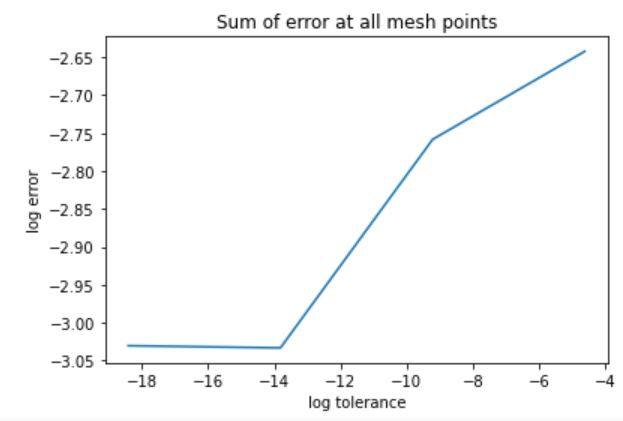
\includegraphics[width=0.95\columnwidth]{ode45_absolute_sum_error_behaviour}
    \caption{Total error of RKF45 method for various absolute tolerance.}
    \label{fig:ode45_absolute_sum_error_behaviour}
\end{figure}

\begin{figure}
    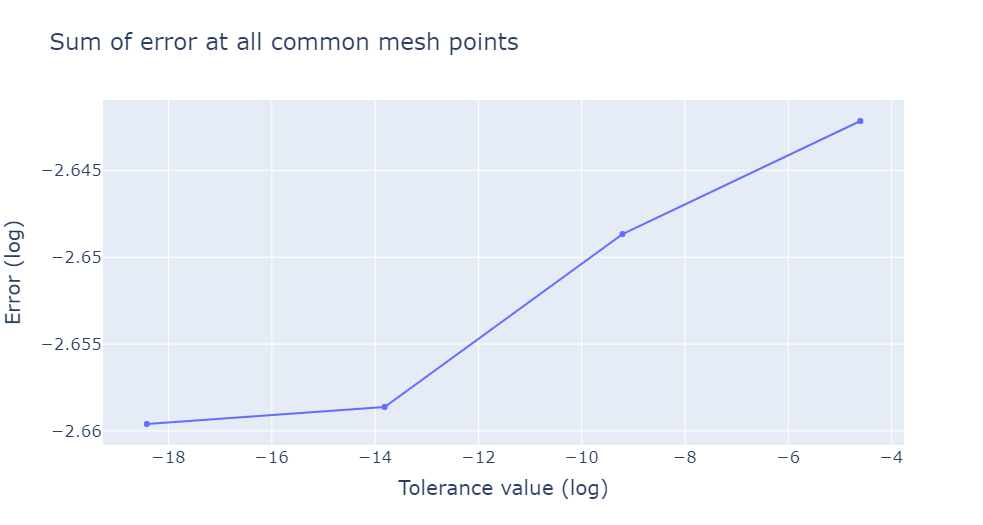
\includegraphics[width=0.95\columnwidth]{ode45_relative_sum_error_behaviour}
    \caption{Total error of RKF45 method for various relative tolerance.}
    \label{fig:ode45_relative_sum_error_behaviour}
\end{figure}